\documentclass[ignorenonframetext,]{beamer}
\setbeamertemplate{caption}[numbered]
\setbeamertemplate{caption label separator}{: }
\setbeamercolor{caption name}{fg=normal text.fg}
\beamertemplatenavigationsymbolsempty
\usepackage{lmodern}
\usepackage{amssymb,amsmath}
\usepackage{ifxetex,ifluatex}
\usepackage{fixltx2e} % provides \textsubscript
\ifnum 0\ifxetex 1\fi\ifluatex 1\fi=0 % if pdftex
  \usepackage[T1]{fontenc}
  \usepackage[utf8]{inputenc}
\else % if luatex or xelatex
  \ifxetex
    \usepackage{mathspec}
  \else
    \usepackage{fontspec}
  \fi
  \defaultfontfeatures{Ligatures=TeX,Scale=MatchLowercase}
\fi
% use upquote if available, for straight quotes in verbatim environments
\IfFileExists{upquote.sty}{\usepackage{upquote}}{}
% use microtype if available
\IfFileExists{microtype.sty}{%
\usepackage{microtype}
\UseMicrotypeSet[protrusion]{basicmath} % disable protrusion for tt fonts
}{}
\newif\ifbibliography
\hypersetup{
            pdftitle={Title},
            pdfborder={0 0 0},
            breaklinks=true}
\urlstyle{same}  % don't use monospace font for urls
\usepackage{graphicx,grffile}
\makeatletter
\def\maxwidth{\ifdim\Gin@nat@width>\linewidth\linewidth\else\Gin@nat@width\fi}
\def\maxheight{\ifdim\Gin@nat@height>\textheight0.8\textheight\else\Gin@nat@height\fi}
\makeatother
% Scale images if necessary, so that they will not overflow the page
% margins by default, and it is still possible to overwrite the defaults
% using explicit options in \includegraphics[width, height, ...]{}
\setkeys{Gin}{width=\maxwidth,height=\maxheight,keepaspectratio}

% Prevent slide breaks in the middle of a paragraph:
\widowpenalties 1 10000
\raggedbottom

\AtBeginPart{
  \let\insertpartnumber\relax
  \let\partname\relax
  \frame{\partpage}
}
\AtBeginSection{
  \ifbibliography
  \else
    \let\insertsectionnumber\relax
    \let\sectionname\relax
    \frame{\sectionpage}
  \fi
}
\AtBeginSubsection{
  \let\insertsubsectionnumber\relax
  \let\subsectionname\relax
  \frame{\subsectionpage}
}

\setlength{\parindent}{0pt}
\setlength{\parskip}{6pt plus 2pt minus 1pt}
\setlength{\emergencystretch}{3em}  % prevent overfull lines
\providecommand{\tightlist}{%
  \setlength{\itemsep}{0pt}\setlength{\parskip}{0pt}}
\setcounter{secnumdepth}{0}

\title{Title}
\date{}

\begin{document}
\frame{\titlepage}

\begin{frame}

class: center, middle \# It is Mixed: \#\# Ambigiouties in digital
(text) analysis Hjalmar Bang Carlsen\\
PhD at the Department of Sociology and Center for Social Data
Science(SODAS),\\
University of Copenhagen\\
hc@soc.ku.dk ??? add some notes --- background-image:
url('/Users/hjalmarbangcarlsen/Dropbox/phd\_project/phd\_project/6. From
Act to Activist/plots/refugees\_on\_the\_highway.jpg') --- class:
center, middle \#\#\# The Growth of the Refugee Solidarity Movement
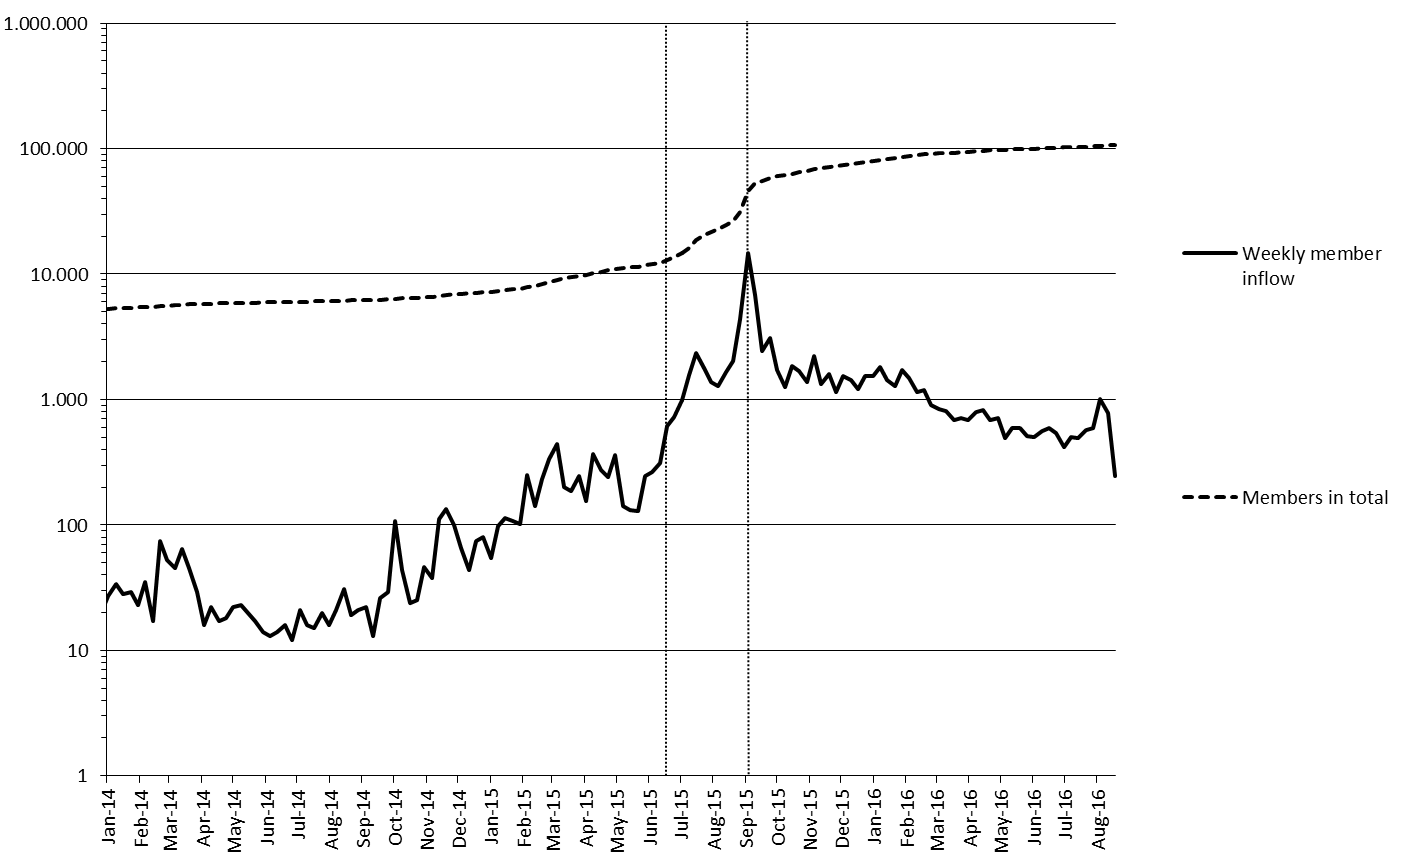
\includegraphics[width=8.33333in,height=5.20833in]{figure1.png} ---
class: center, middle \#\#\# Two different activist styles
\includegraphics[width=4.16667in,height=3.12500in]{anne_mette\&Magrete.jpeg}
``*The immigration office should be called the office for second-rate
citizens*'' ``*The journalist does say that the Friendly People fight
FOR something - not AGAINST something. In fact, it should NOT read
`fight' - because we don't fight❤️ This is precisely what should
characterize the values of the Friendly People. Fighting creates
resistance! And resistance is not appropriate if you want change🍃*'' ---
class: center, middle Why did the Refugee Solidarity Movement remain
uncontentious although all conditions for politicalization and
radicalization where present? (a highly contentious environment,
socialization with likeminded others) --- class: center, middle
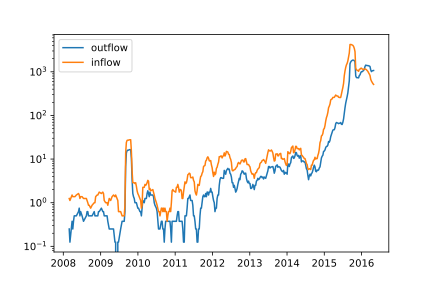
\includegraphics[width=7.29167in,height=7.29167in]{outflow_inflow.svg}
--- class: center, middle
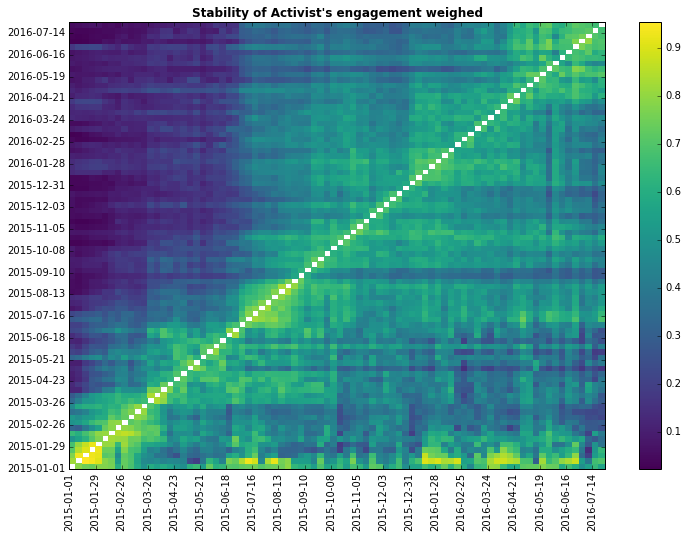
\includegraphics[width=7.29167in,height=6.25000in]{stability_of_activist_engagement.png
} --- class: center, middle
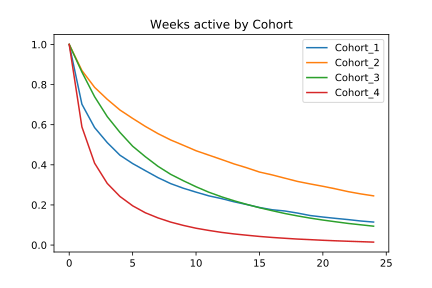
\includegraphics[width=7.29167in,height=6.25000in]{Survival function of Activist by Gender.svg}
--- class: center, middle \#\# Enriching poor activity with rich textual
data \{Some cartoon gif where a throught boble is connected to characher
walking\} --- class: center, middle How do reduce and categorises
750.000 million different communications acts into interpretable,
usefull and valid data? ---

\end{frame}

\end{document}
